\paragraph{Marking}

\begin{figure}[ht]
    \centering
    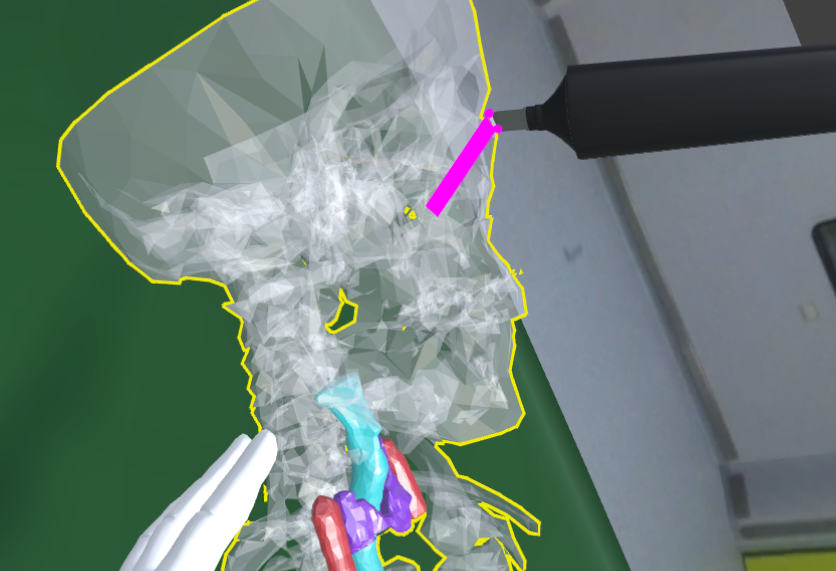
\includegraphics[width=\linewidth]{images/implementation/features/procedures/marker.png}
    \caption{\label{fig::FeatureMarker}Marker procedure. The marker is hold in such a way that it does not occlude the users view while performing the marking procedure.}
\end{figure}

The \textbf{marking} procedure is similar to the bonesaw procedure, meaning that rectangular shapes are drawn into the three dimensianal space (Figure \ref{fig::FeatureMarker}).
However, here the created shapes are much thinner.
In contrast to the bonesaw, the virtual hands of the user are also disabled here.
This way, the user can decide to hold the marker in the optimal way.
Another reason to deactivate the user's hand on the virtual marker was that since the marker is relatively thin, the virtual hands negatively impacted the users viewpoint.
Since the main objective is marking specific spots on the patient, this is the natural approach.